\documentclass[12pt,a4paper]{report}

\usepackage[english]{babel}
\usepackage{datetime}
\usepackage[hidelinks]{hyperref}
\usepackage{longtable}
\usepackage{lipsum}
\usepackage{amsthm}
\usepackage{listings}
\usepackage{graphicx}
\usepackage{pdfpages}
\usepackage{wasysym}


\lstset{basicstyle=\ttfamily,breaklines=true}

\newtheorem{theorem}{Theorem}[section]
\theoremstyle{definition}
\newtheorem{exercise}[theorem]{Exercise}
\newtheorem{myrule}{Rule}


\title{Prototype Verification System

{\large Lecture Notes}}
\author{Daniele Parmeggiani}


\newdate{today}{29}{02}{2024}
\date{\usdate\displaydate{today}}


\begin{document}
\maketitle

\tableofcontents

\chapter{Introduction}

In this chapter we will introduce PVS (the Prototype Verification System),\footnote{%
	\url{https://pvs.csl.sri.com/}
} and we will install a modern environment for using PVS.
Later, we'll also see how to prove some simple properties of a hashmap using PVS.


\section{Introduction to PVS}

PVS is a powerful tool designed for formal specification and verification of software and hardware systems.
It is a language coupled with a complete environment for developing formal mathematical specifications and then verifying that those meet certain properties.

PVS comes with an expressive specification language that allows you to describe your systems in a precise and formal manner.
One of the core functionalities of PVS is its ability to prove theorems about your specifications.
This involves using mathematical reasoning to demonstrate that certain properties hold true for your system under specified conditions.

PVS includes a set of built-in libraries that cover a wide range of mathematical theories and common programming constructs. 
These libraries provide a foundation for specifying and verifying a variety of systems.
Notably among them, we can find NASALib,\footnote{%
	\url{https://github.com/nasa/pvslib}
} a vast set of libraries developed by the Formal Methods teams at the NASA Langley Research Center, along with the Stanford Research Institute, the National Institute of Aerospace, and the larger PVS community.

PVS is often used to verify critical software systems where correctness is of utmost importance, such as avionics and aerospace software, medical devices, or other safety-critical applications.

It is also extensively employed in the verification of hardware systems, and can be used to formally specify and verify communication protocols, cryptographic and concurrent algorithms, and other complex systems.


\section{Installing PVS}

The recommended development environment for PVS is NASA's plugin for Visual Studio Code:\footnote{%
	\url{https://github.com/nasa/vscode-pvs}
}

\begin{enumerate}
	\item download and install Visual Studio Code for your platform from \url{https://code.visualstudio.com/download};
	\item navigate to the extensions tab in VS Code (the blocks icon at the left edge of the screen) and search for ``pvs'';
	\item the first item in the list should be called ``PVS'' and authored by Paolo Masci;
	\item click the install button and follow the on-screen installation instructions.
\end{enumerate}

Note that this procedure installs the PVS binaries and libraries in your system as well, at a path that you need to specify.

To confirm that everything was installed correctly, open a new VS Code workspace; i.e. create and select a folder from your file system.
Then, navigate to the newly appeared PVS tab at the left edge of the screen, right-click on the folder's name and select ``New PVS File.''
In the new file insert the following content:

\begin{verbatim}
	hello: THEORY
	  BEGIN

	  world: CONJECTURE
	    TRUE
	END hello
\end{verbatim}

Now, right-click the name of the new file on the left panel and select ``Re-run All Proofs:'' you should see a new tab called \texttt{hello.summary} displaying the above conjecture \texttt{world} with the status \texttt{proved}.

For further help installing this plugin, please refer to \url{https://github.com/nasa/vscode-pvs#installation-instructions}.


\section{Proving Properties of a Hashmap}

Let us introduce the core concepts and features of the PVS proof assistant with a commonly known data structure. We will try to prove a hashmap has the following features:

\begin{enumerate}
	\item it should be possible to insert a new (key, value) pair;
	\item it should be possible, given a key, to retrieve its corresponding value; and
	\item it should be possible to remove a (key, value) pair from the hashmap.
\end{enumerate}

Let's name these operations \emph{insert}, \emph{lookup}, and \emph{delete}.
Since we'll be talking about keys, values and maps, we should let PVS know about them.
Specifically, we introduce new \emph{uninterpreted} types; i.e. types that PVS knows nothing about: whether there would be 0, 1, or infinite instances of these types, for example.
PVS instead is thus only told that a key \texttt{K} is something different from a value \texttt{V}.

\begin{verbatim}
	K: TYPE
	V: TYPE
\end{verbatim}

Now we define what a hashmap is, and we use this notation:

\begin{verbatim}
	M: TYPE = [K -> V]
\end{verbatim}

This tells PVS that a hashmap \texttt{M} is a function from keys to values.
We will later define this function as a sequence of associations.
You can also think of this \texttt{TYPE} as an array of (key, value) pairs.\footnote{%
	PVS also allows expressing exactly \emph{an array of tuples}, but it's able to reason very efficiently with functions, which is why we choose this representation.
}

We could define \texttt{M} as a partial function (that is, a function defined over a subset of its domain), but efficient theorem proving strongly encourages the use of total functions.
One way to denote the fact that some $k \in K$ is not to be found in the hashmap, is to identify some particular value that indicates this.
Let's choose an arbitrary element of \texttt{V}:

\begin{verbatim}
	null: V
\end{verbatim}

So that, we will expect a hashmap to be empty iff $\forall k \in K, m(k) = \texttt{null}$.
We can write this in PVS too:

\begin{verbatim}
	empty: M
	empty_ax: AXIOM
	    FORALL (k: K): empty(k) = null
\end{verbatim}

We have declared a hashmap to be the \emph{one} empty hashmap, and we have axiomatically defined \texttt{empty} as the hashmap in which all keys point to \texttt{null}.
This may surprise a programmer who's used to think that there may be multiple instances of a hashmap class that all happen to be empty.
From the point of view of PVS, though, all those instances are exactly the same.
A program may distinguish them based on their memory address, but PVS has no notion of this, instead it only knows abstractly about the types we have defined so far.
Think of it mathematically instead of programmatically: the number 0 is exactly the number 0 no matter how many times we may write it on a piece of paper.

Also, do not consider the axiom itself to be computationally expensive since it associates \texttt{null} to the entire key space.
Quite the contrary: in the carrying out of a proof, PVS will know that whatever we may write next, the value of any key in \texttt{empty} will be \texttt{null}, without employing any memory to store the possible associations.

Now, let's ``implement'' the hashmap operations:

\begin{verbatim}
	lookup: [M, K -> V]
	lookup_ax: AXIOM FORALL (m: M) (k: K):
	    lookup(m, k) = m(k)
	
	insert: [M, K, V -> M]
	insert_ax: AXIOM FORALL (m: M) (k: K) (v: V):
	    insert(m, k, v) = m WITH [(k) := v]
	
	delete: [M, K -> M]
	delete_ax: AXIOM FORALL (m: M) (k: K):
	    delete(m, k) = m WITH [(k) := null]
\end{verbatim}

Notice some of the notations we have used so far: \texttt{m(k)} is exactly equivalent to the mathematical notation of function application, the \texttt{AXIOM} and \texttt{FORALL} keywords refer to their usual meanings, and the keyword \texttt{WITH} has been used to add an association to the function \texttt{m} above.

Also, notice the \emph{functional} specification style: we pass the whole ``state of the system'' (i.e. the entire hashmap) to the functions \texttt{lookup}, \texttt{insert}, and \texttt{delete}.
Consider \texttt{insert}: the input hashmap is somehow discarded in the operation and we instead ``return'' a novel hashmap that has the added association.
As previously said, do not consider that PVS will actually allocate and deallocate memory to represent these hashmaps.

If we were programming a hashmap and we felt content of what we wrote, we may turn to writing tests.
But with PVS we instead want to write theorems about our hashmaps: they are general statements that we think should be true if our specification does what it ought to.
This can provide much more information than a single test case, since with one theorem we would be running an entire \emph{class} of test cases.

A suitable challenge for our specification may be: ``if I add a key \texttt{k} with a value \texttt{v} to a hashmap and then I lookup \texttt{k}, I should get back \texttt{v}.''
We can write it as:

\begin{verbatim}
	insert_then_lookup: CONJECTURE FORALL (m: M) (k: K) (v: V):
	    lookup(insert(m, k, v), k) = v
\end{verbatim}

In your VS Code editor, you should see some links above the definition of \texttt{insert\_then\_lookup}. We invoke the prover by clicking ``prove'':

\begin{verbatim}
	Starting prover session for insert_then_lookup
	
	
	insert_then_lookup :
	
	|-------
	{1}   FORALL (m: M) (k: K) (v: V): lookup(insert(m, k, v), k) =
	v
	
	>>  
\end{verbatim}

This is a \emph{sequent}: in general there will be several numbered formulas above the turnstile symbol \texttt{|-------} (antecedent), and several below (consequent).
The idea is that we have to establish that the conjunction (and) of formulas in the antecedent implies the disjunction (or) of the formulas in the consequent.
Therefore, a sequent is true if any antecedent is the same as any consequent, if any antecedent is false, or if any consequent is true.

The prompt indicates that PVS is waiting for us to submit a prover command, in Lisp syntax.
The commands provided by PVS can be categorized as basic commands and strategies, which in turn are compositions of basic commands.
Let us disregard enumerating all of the various commands available and their semantics during this introduction (they will be explored later in \S ???) and let us instead introduce a few commands and consider how a proof with PVS can be carried out in general.

The highest-level strategy is called \texttt{grind}. It does skolemization, heuristic instantiation, propositional simplification, if-lifting, rewriting, and applies decision procedures for linear arithmetic and equality.
It can take several optional arguments to specify the formulas that can be used for automatic rewriting (below, we'll be specifying that it can use the axioms in the theory \texttt{hashmap}).

Following the execution of a command, PVS may be required to split the proof into two or more parts.
The PVS prover itself maintains a proof tree; the act of proving the specification can be thought of as traversing the tree, with the goal of showing that each leaf of the tree is true.

The \texttt{grind} strategy satisfies the proof for \texttt{insert\_then\_lookup}:

\begin{verbatim}
	>> (grind :theories ("hashmap"))
	
	Q.E.D.
\end{verbatim}

Following the display of \texttt{Q.E.D.}, you should see a pop-up indicating that the proof has been saved.
We will mostly run our proofs in the interactive environment, but after a proof is successfully completed, it can be re-run in batch mode, without user interactions.
Interactive proofs can also be suspended with \texttt{(quit)} and later resumed.

In the example shown above the proof tree had just one trivial branch. Now let's turn to another less trivial conjecture:

\begin{verbatim}
	insert_then_delete: CONJECTURE FORALL (m: M), (k: K), (v: V):
	    delete(insert(m, k, v), k) = m
\end{verbatim}

Intuitively, the above states that inserting a key \texttt{k} into a hashmap \texttt{m} and then deleting \texttt{k}, yields \texttt{m} unchanged.
The first proof went very smoothly, let's see about this one.
The same strategy used before produces the following result:


\begin{verbatim}
	Starting prover session for insert_then_delete
	
	
	insert_then_delete :
	
	|------- 
	{1}   FORALL (m: M), (k: K), (v: V): delete(insert(m, k, v), k)
	= m
	
	>> (grind :theories ("hashmap"))
	
	
	Trying repeated skolemization, instantiation, and if-lifting
	
	insert_then_delete :
	
	|-------
	{1}   m!1 WITH [(k!1) := null] = m!1
	
	>> 
\end{verbatim}

The identifiers with \texttt{!} in them are Skolem constants---arbitrary representatives for quantified variables.
Notice that PVS has already simplified away one of the two \texttt{WITH} expressions: if it only substituted the axioms, it could have equivalently written \texttt{m!1 WITH [(k!1) := v!1] WITH [(k!1) := null] = m!1}.

The resulting sequent is requesting us to prove that two functions (i.e. hashmaps) are equal.
We try to appeal to the principle of extensionality, which states that two functions are equal if their values are the same for every point of their domains:

\begin{verbatim}
	>> (apply-extensionality)
	
	
	Applying extensionality
	
	insert_then_delete :
	
	|-------
	{1}   m!1 WITH [(k!1) := null](x!1) = m!1(x!1)
	[2]   m!1 WITH [(k!1) := null] = m!1
	
	>> (delete 2)
	
	
	Deleting some formulas
	
	insert_then_delete :
	
	|-------
	[1]   m!1 WITH [(k!1) := null](x!1) = m!1(x!1)
	
	>> 
\end{verbatim}

At any point we can invoke the \texttt{delete} command to remove an element of a sequent; here the original formula was deleted to reduce clutter, since it is equivalent to the  more interesting extensional form.\footnote{%
	Recall that to prove a sequent we need to prove that the conjunction of the antecedents implies the disjunction of the consequents.
}

This sequent is asking us to show that the value associated with an arbitrary key \texttt{x!1} is the same before and after \texttt{m} was updated for \texttt{k!1}.
We can do a case analysis here to consider whether $\texttt{x!1} = \texttt{k!1}$.

\begin{verbatim}
	>> (lift-if)
	
	
	Lifting IF-conditions to the top level
	
	insert_then_delete :
	
	|-------
	{1}   IF x!1 = k!1 THEN null = m!1(x!1) ELSE TRUE ENDIF
	
	>> (ground)
	
	
	Applying propositional simplification and decision procedures
	
	insert_then_delete :
	
	{-1}   x!1 = k!1
	|-------
	{1}   null = m!1(x!1)
	
	>> 
\end{verbatim}

Let's look closely at this sequent: it is asking to demonstrate that if $x_1 = k_1$, then $m_1(x_1) = \texttt{null}$, but modus ponens, we also are trying to show that $m_1(k_1) = \texttt{null}$.
That is, that the hashmap's value for $k_1$ was \texttt{null} before we inserted $k_1$.
But it doesn't necessarily have to be so!
If the value associated with $k_1$ was a non-null value, say $v_2$, then the \texttt{insert} operation \emph{updates} the association and the later \texttt{delete} associates $k_1$ to \texttt{null}.
Thus, our conjecture (that the hashmap is unchanged following an \texttt{insert} + \texttt{delete}) is true only under the assumption that the key we add to the hashmap wasn't already in the hashmap (i.e. $m(k) = \texttt{null}$).

If we change our conjecture to
\begin{verbatim}
	insert_then_delete: CONJECTURE FORALL (m: M), (k: K), (v: V):
	    lookup(m, k) = null => delete(insert(m, k, v), k) = m
\end{verbatim}
then, we can prove it with
\begin{verbatim}
	(grind :theories ("hashmap"))
	(apply-extensionality)
	(delete 2)
	(grind :theories ("hashmap"))
\end{verbatim}


\subsection{Axiomatic Issues}

Let's now introduce two seemingly innocuous axioms, extending our specification the same way we have done before:

\begin{verbatim}
	is_in?: [M, K -> bool]
	is_in_ax: AXIOM FORALL (m: M), (k: K):
	    m(k) /= null
	
	insert_is_in_ax: AXIOM FORALL (m: M), (k: K), (v: V):
	    is_in?(insert(m, k, v), k)
\end{verbatim}

The semantics of these axioms should be fairly self-explanatory: a key is in the hashmap if it is not null, and after inserting some key $k$ in a hashmap \texttt{m}, \texttt{k} is in \texttt{m}.

But these axioms hide an inconsistency!

\begin{exercise}
	Prove, without using PVS, that true = false, based on the axioms provided so far.
	
	\emph{Hint}: start from \texttt{is\_in?(insert(empty, k, null), k)}.
\end{exercise}

In fact, it shouldn't be possible that after associating a key $k$ with \texttt{null}, we find that the value associated with $k$ is not \texttt{null}!
We have clearly abused axiomatic definitions and PVS will happily run this impossible proof for us, given that the inconsistency is within the axioms themselves, that PVS assumes to hold.
We'll see later how to avoid abusing axioms, but for now, let's try to carry out the exercise proof using PVS.

\begin{verbatim}
	Starting prover session for what
	
	
	what :
	
	|-------
	{1}   FORALL (k: K): is_in?(insert(empty, k, null), k)
	
	>> (skolem!)
	
	
	Skolemizing
	
	what :
	
	|-------
	{1}   is_in?(insert(empty, k!1, null), k!1)
	
	>> (use "insert_ax")
	
	
	Using lemma insert_ax
	
	what :
	
	{-1}   insert(empty, k!1, null) = empty WITH [(k!1) := null]
	|-------
	[1]   is_in?(insert(empty, k!1, null), k!1)
	
	>> (use "is_in_ax")
	
	
	Using lemma is_in_ax
	
	what :
	
	{-1}   insert(empty, k!1, null)(k!1) /= null
	[-2]   insert(empty, k!1, null) = empty WITH [(k!1) := null]
	|-------
	[1]   is_in?(insert(empty, k!1, null), k!1)
	
	>> (use "empty_ax")
	
	
	Using lemma empty_ax
	
	what :
	
	{-1}   empty(k!1) = null
	[-2]   insert(empty, k!1, null)(k!1) /= null
	[-3]   insert(empty, k!1, null) = empty WITH [(k!1) := null]
	|-------
	[1]   is_in?(insert(empty, k!1, null), k!1)
	
	>> (ground)
	
	Q.E.D.
\end{verbatim}

The complete \texttt{.pvs} file for this example can be found in \S\ref{sol:simple-hashmap}.


\section{Exercises}

\begin{exercise}\label{ex:chapter1-1}
	Encode in PVS grammar the following properties of natural numbers, without proving them.
	Note that in PVS to denote that a variable is a natural number, we write e.g. \texttt{FORALL (n: nat)}.
	
	\begin{enumerate}
		\item Let $n \in \mathbf{N}$, $n > 5 \Rightarrow n > 10$.
		
		\item Let $x, y, z \in \mathbf{N}$. If $x = y + z$, then $x^2 = yx + zx$, $xy = y^2 + zy$, and $xz = z^2 + yz$.
		
		\item Let $x, y, z \in \mathbf{N}$. If $x = y + z$ and the above formulae hold, then $x^2 = y^2 + z^2 + 2yz$, and $(y + z)^2 = y^2 + z^2 + 2yz$.
	\end{enumerate}

	What happens when you try to prove these properties using \texttt{(grind)}?
\end{exercise}

%\begin{longtable}{p{.5\textwidth}p{.5\textwidth}} 
%	\texttt{\lipsum[1]} & \lipsum[2] \\
%\end{longtable}


\chapter{Fundamentals of PVS Syntax and its Prover}

You can read more on the ``PVS Language Reference'' (Owre et al., 2020) and the ``PVS Prover Guide'' (Shankar et al., 2020).

A language cheat-sheet can be found in Appendix~\ref{ch:cheatsheet}.

\chapter{Concurrent Reference Counting}\label{ch:concurrent-reference-counting}

Let us now go through a more interesting specification: one that deals with concurrent memory management.
In this chapter we'll practice ...

As a basis, we observe that computer memory is an array of bytes.
On a 64-bit computer, you can address memory from byte number 0, to byte number $2^{64} - 1$.
This is not a simplistic assumption that we're making here: it's the abstraction that all modern computers and operating systems use.
Of course, memory is more complicated than this: there is virtual memory, kernel-space memory, file-system mapped memory, and process-specific memory, to name a few.

In here, we cannot go in so deep as to take all of these different kinds of memory into consideration.
Instead, we'll be specifying the memory for one single process, as if all the rest is not there.

Another assumption we'll make is that the machine memory is unbound\-ed.
This sort of makes memory management redundant, but here we're interested in specifying the behavior of a management system irrespective of the amount of memory it can dispose of.

We can be free to add this constraint later, and we will, after we dealt with the other issues that will come up shortly.

To keep things simple, we'll specify a reference counting-based, object-oriented scheme.
That is, we assume that our model process has knowledge of thing called objects, that may represent different classes of data.
In managing memory, though, what the classes of data are isn't important.
Each object has an amount of memory associated with it and however large or small it may be, we can assume the correct amount will be allocated (because we assumed memory is infinite), and deallocated once the object is freed.

\section{Specification}\label{sec:specification}

The following rules are the behavior of the memory management system we would like to specify:

\begin{myrule}\label{refcount:allocate-1}
	When an object is allocated, its reference count will be 1.
\end{myrule}

\begin{myrule}\label{refcount:free-when-0}
	Any object can be freed if its reference count is 0.
\end{myrule}

\begin{myrule}\label{refcount:incref}
	When a new reference is made to an existing object, the object's reference count must be increased by 1.
\end{myrule}

\begin{myrule}\label{refcount:decref}
	When an existing reference to an object is removed, the object's reference count must be decreased by 1.
\end{myrule}

The rules, that will be verified, are based on these intuitive notions:
\begin{enumerate}
	\item when an object is allocated, the returned pointer is the only reference to that object;
	\item such is the case when no other object or variable is referencing it, thus it is safe to reclaim the memory;
	\item[3-4.] the stored reference count must be kept consistent with its semantics.
\end{enumerate}

The rules above ensure essentially that, in principle, any allocated object can be eventually freed, when its presence is no longer necessary.

Notice though, how Rule~(\ref{refcount:free-when-0}) doesn't specify that the object \emph{is} freed, only that it \emph{can} be freed.
This will become important later, but first we need to talk about why these properties alone are not sufficient.

There are important features of a memory management system that we're not guaranteeing: eventual reclamation, and use-after-free avoidance.
As already stated, Rule~(\ref{refcount:free-when-0}) only requires the possibility of freeing; we want to enforce that an object that can be freed, will be freed.

Use-after-free is a commonly known bug of programs that don't employ a memory management system, or that use it incorrectly.
What happens is that a piece of memory is freed and then used again, as the name implies, either for a read or for a write.
At that point, the program generally crashes with a segmentation fault.
A more subtle, but possibly worse, manifestation of this bug is when the program requests to allocate memory and the allocation routine returns some address $x$, the program then frees $x$, requests more memory to be allocated, and the allocation routine returns $x$ again.\footnote{%
	This is not an unlikely scenario, many memory management systems allocate chunks of memory.
	When a call to the free routine is made, the system marks that piece of memory within a chunk as free, and when a successive call to the allocation routine for the same size is made, the previously freed piece is unmarked and returned.
	
	This behavior is useful to improve performance by not continuously relying on calls to the kernel when allocations are frequent.
	Object-oriented and functional language runtimes often exhibit this usage pattern.
}
If we distinguish the two states of the object at $x$ with $A$ and $B$, we may be surprised when using the pointer $x$ as if it was $A$, but instead it is $B$.
This may not be a problem per se, but generally can be a very tricky situation in a concurrent system.
In fact it could be that one thread $t_1$ frees $A$ and allocates an unrelated object $B$, while another thread $t_2$ still had a pointer $x$ that it considered to pertain to $A$.
This of course is a bug in the overall program.
In a reference count-based memory scheme, a possible cause of such a bug is that the code of $t_2$ didn't correctly account for a new reference to $A$, or that $t_1$ incorrectly decremented the reference count.

Let us add more rules to deal with these problems.

% Since we're dealing with the verification of this kind of system, we will deal with an idealized usage, rather than a realistic case: we cannot possibly enumerate all usages.
% Nevertheless, we still need to prove that the idealized usage, introduced later, is correct: it cannot lead to a program that uses memory previously reclaimed.


\begin{myrule}\label{refcount:0-stays-0}
	When the reference count of an object is 0, it remains 0 until the object is freed.
\end{myrule}

\begin{myrule}\label{refcount:free-implies-0}
	If an object is being freed, its reference count must be 0.
\end{myrule}

\begin{myrule}\label{refcount:use-after-free}
	If an object has been freed, no thread tries to use it.
\end{myrule}

\begin{myrule}\label{refcount:eventual-free}
	After the reference count of an object becomes 0,\footnote{%
		Such is a definite, unique point in the program execution due to the combination of Rules~(\ref{refcount:allocate-1}), and (\ref{refcount:0-stays-0}).
	} the object is eventually freed.
\end{myrule}

\section{Pseudocode}\label{sec:pseudocode}

In this section we'll be constructing a program in C-like pseudocode to use as a reference for what we intend to specify later in PVS\@.
Some base-level C knowledge is required to read this section.

First, we can easily declare our object, which we'll be using throughout our pseudocode.

\begin{verbatim}
	typedef struct {
	    int refcount;
	    bool allocated;
	    bool freed;
	} object;
\end{verbatim}

It is a very simple abstraction for an object.
Remember as we've said previously, we don't want to actually store any kind of data in this object.
We'll be doing it later.
So, for now, we only care about an object's reference count (the \texttt{refcount} field).
We also add two flags which are only used to simplify our specification: in a real system the fact that a portion of memory is allocated or free is stored in kernel data structures (and possibly also in user-space when a memory management system is employed).
We do not care about those details here.
Instead, we attach this information to the objects themselves.
It would be of course a significant waste in space, but we have an infinite amount of it here ;)

Next, we'll be doing something weird.
Each thread has its own set of registers, which we can imagine as its current view of the shared memory.
As you may know, in C there is no direct access to registers,\footnote{%
	Unless you embed assembly code.
} the mapping of variables to registers is left to the compiler.
So, in order to make clear the usage of registers by a thread, we introduce an explicit \texttt{registers} array:
\begin{verbatim}
	object *registers[10] = {NULL, NULL, NULL, NULL,
	    NULL, NULL, NULL, NULL, NULL, NULL};
\end{verbatim}

Another thing we generally don't get to see is the stack.
Memory on the heap is explicitly allocated in a C program, but not the variables that are allocated onto the stack.
Again, we want to make it clear that a thread is viewing a certain set of variables:
\begin{verbatim}
	object *variables[10] = {NULL, NULL, NULL, NULL,
	    NULL, NULL, NULL, NULL, NULL, NULL};
\end{verbatim}

Both of these arrays should be thought of as thread-local storage, with each thread seeing a different array.
This is implicit in the pseudo program, because we avoid explicitly starting threads.

With the above definition of an object, the \texttt{free} routine becomes straight-forward, beacuse we just need to set the \texttt{freed} flag:
\begin{verbatim}
	void free()
	{
	    CAS(registers[0]->freed, false, true);
	}
\end{verbatim}

There are a couple of things to note here.
First, we're using a \texttt{CAS} function, which we don't declare nor define, that denotes the usage of a hardware compare-and-set instruction to perform this write to memory.
This pseudo-function returns a boolean value, which we just don't care to look at here.
We'll take care of the fact that the object wasn't already freed by other means.

Second, this routine takes no input parameters, while the usual C \texttt{free} function does require the pointer to the memory that needs to be freed.
Here, we're making a choice to simplify further the PVS specification that will follow.
Instead of specifying that there is a parameter, we assume that the parameter is in register number 0.
Note that this is not a PVS-specific way of doing this, we're just making this deliberate choice on how we model a real program execution.

Next, the allocation routine:
\begin{verbatim}
	void alloc()
	{
	    do {
	        object *obj = choose();
	    } while (!CAS(obj->allocated, false, true));
	    obj->refcount = 1;
	    registers[0] = obj;
	}
\end{verbatim}

Weirdness abounds.
Let's break it down.
First, the signature is again unexpected.
Again, the reason is simplifying the PVS specification: instead of specifying a return mechanism we rely on the assumption that the returned value is found in register number 0, instead of actually modeling the return register.

Then, what's that \texttt{choose()} doing?
As said, \texttt{malloc} and the like have special data structures that are used to determine which address in memory is the next free address that can be allocated, but we don't care to map it to our specification.
So, instead, we ``choose'' an address.
That is, we \emph{non-deterministically} pick one at random until we find an object that wasn't already allocated.
Non-determinism is certainly not a characteristic usually found in computer programs.
You can think of it as a non-deterministic Turing machine that outputs a random address.
With non-determinism, we can also ``be lucky'' and find a non-allocated object on our first try.
Which is exactly what we'll do later in the PVS specification.
Here, the check inside the while is kept in order to be clear about the state of \texttt{obj} after the loop.

Now we define the reference count increment and decrement routines, and we'll look at them together, given that they're pretty similar:
\begin{verbatim}
	void inc_ref()
	{
	    object *obj = registers[0];

	    do {
	        int refcount = obj->refcount;  // registers[1]

	        if (obj->refcount == 0) {
	            registers[0] = NULL;
	            return;
	        }
	    } while (!CAS(obj->refcount, refcount, refcount + 1));
	}

	void dec_ref()
	{
	    object *obj = registers[0];

	    do {
	        int refcount = obj->refcount;

	        if (obj->refcount == 0) {
	            registers[0] = NULL;
	            return;
	        }
	    } while (!CAS(obj->refcount, refcount, refcount - 1));
	    refcount--;

	    if (refcount == 0) {
	        free(obj);
	    }
	}
\end{verbatim}

These two routines shouldn't be very surprising, given what we've already seen so far.
In both, we read the current reference count of the input object and attempt to modify it accordingly.
In case we fail, because another thread modified the count concurrently, we read it again and retry.
This should be the expected way to correctly implement a concurrent counter.

The decrement routine also takes care of freeing the object in case its reference count reaches 0.
This leads to a subtle problem.
Consider this execution: two threads $t_1$ and $t_2$ are respectively trying to incref and decref a shared object $x$.
Both read $\mathrm{refcount}(x) = 1$.
$t_2$ proceeds before $t_1$ and decrements the reference count.
Additionally, $t_2$ executes the call to \texttt{free} before $t_1$ attempts to CAS the reference count.
The object has thus been freed before $t_1$ executes the CAS\@.
When $t_1$ tries to execute the CAS, it breaks Rule~(\ref{refcount:use-after-free}).

We have thus determined that the decref routine cannot also take care of freeing the object that has reached a reference count of 0.
In fact, if it was also done inside the same routine, the thread executing it would need to wait for an indefinite amount of time before executing free.
Instead, we'll employ a scheme known as Quiescent State Based Reclamation (QSBR): we'll defer the call to free until we know no thread is trying to access objects that have $\mathrm{refcount}(x) = 0$.
That is, we need a Garbage Collector (GC).

Instead of calling \texttt{free} in \texttt{dec\_ref}, we append the decref'ed object to a GC tracking list.
When the GC will run a collection cycle, the tracked objects will be freed.

Let's add the GC structures at the top of our pseudocode:
\begin{verbatim}
	extern int T;  // number of threads (T >= 1)

	// ...

	typedef struct GC {
	    object *obj;
	    struct GC *next;
	} GC;

	GC *gc_head = NULL;
	bool STW_world_stopped = false;  // stop the world
	bool STW_requested = false;
	int STW_count_down = T;
\end{verbatim}

As you can already see, we'll be implementing a very simple stop-the-world GC later, based on a single linked list of tracked objects to be freed.
For now, the result is that inside the \texttt{dec\_ref} function we replace the call to free with the following linked-list append:
\begin{verbatim}
	GC *gc = new GC();

	gc->obj = obj;
	gc->next = NULL;

	do {
	    gc_tail = gc_head;
	    while (gc_tail != NULL) {
	        gc_tail = gc_tail->next;
	    }
	} while (!CAS(gc_tail->next, NULL, gc);
\end{verbatim}

A very simple GC cycle can be implemented like this:
\begin{verbatim}
	void collect()
	{
	    GC *gc = gc_head;

	    while (gc != NULL) {
	        free(gc->obj);
	        gc = gc->next;
	    }

	    gc_head = NULL;
	}
\end{verbatim}

As you can see, it's a very trivial list traversal algorithm which calls \texttt{free}.
The complexity will stem from the stop-the-world part of this GC\@.
When a thread becomes the GC (i.e.\ initiates a GC cycle), it will need to make sure that no other thread is executing an incref or a decref.
As said, it will do so by locking all other threads out of execution.
The mechanism is not very complicated: first we signal all threads that a stop-the-world (STW) request has occurred, then we wait for all other threads to acknowledge the request, and finally we signal that we have successfully stopped the world.
After the call to collect completes, we reset the STW state.
\begin{verbatim}
	void gc_cycle()
	{
	    if (!CAS(STW_requested, false, true)) {
	        return;
	    }

	    while (STW_count_down - 1 > 0) { }  // wait for all threads
	                                        // (except this one)
	    STW_world_stopped = true;

	    collect();

	    STW_count_down = T;
	    STW_requested = false;
	    STW_world_stopped = false;  // resume the world
	                                // (must be last)
	}
\end{verbatim}

\begin{exercise}
	Based on the above \texttt{gc\_cycle} routine come up with a \texttt{STW\_wait} routine, in pseudocode, that performs its counterpart: it is called by all the threads that did not attempt to request a STW operation, and possibly makes them wait for the STW operation to complete before returning.
	A solution can be found in~\S\ref{sec:refcount-full-pseudocode}.
\end{exercise}

Finally, we need to write a \texttt{main} function that is the entry point of all threads.
Again, we're not going to explicitly start any thread, we simply assume that $T$ threads start executing the \texttt{main} function.
In particular, we want it to be an infinite loop over the possible operations that a thread can do: allocate, decref, or incref an object, or start a GC cycle.
No program would exactly behave like this, but this is a close-enough model.
A real program would have some possibly complicated logic on what actions it needs to take, but from the point of view of a memory management system, all that logic is transparent.
Such system would only be able to observe the program continuously requesting one of those operations that we just mentioned.
Therefore, a \texttt{while (true) \{ switch (operation) \{\ldots\} \}} loop is already a sufficiently detailed representation of a program that uses our concurrent memory management system.
Thus, the beginning of our \texttt{main} function can look like this:
\begin{verbatim}
	int main()
	{
	    while (true) {
	        STW_wait();  // maybe wait if the world is stopped,
	                     // or if a stop is requested

	        int action = choose();  // registers[5]
	        int variable = choose();  // registers[6]

	        switch (action) {
\end{verbatim}

We make again use of non-determinism: the action and the variable upon which the action is performed are chosen at random.
For our purposes, this pseudocode maps to a situation in which PVS needs to make sure that our proofs hold for whichever value \texttt{action} and \texttt{variable} may take, which is exactly what we want.
Next we go through the four possible actions: \texttt{alloc}, \texttt{dec\_ref}, \texttt{inc\_ref}, and \texttt{GC}.
The order in which we do so, and the integer numbers we map the actions to, is completely arbitrary.
\begin{verbatim}
	case 1:  // dec_ref
	    if (variables[variable] == NULL) {
	        break;
	    }

	    registers[0] = variables[variable];
	    dec_ref();

	    if (registers[0] == NULL) {
	        goto error;
	    }

	    variables[variable] = NULL;
	    registers[0] = NULL;
	    break;
\end{verbatim}

Notice how we first check that the chosen variable makes sense: that it actually holds a reference to an object.
Given that we're using non-determinism, we need to make sure that we didn't non-deterministically choose something that would break our logic.
In this case, we don't want to decref \texttt{NULL}.
Then, in keeping with our calling convention, we populate register 0 to pass the argument to the \texttt{dec\_ref} function.
If it returned \texttt{NULL}, it means that the reference count of the object in our variables registry reached 0 before the \texttt{dec\_ref} routine could decrement it.
This is considered an impossibility: how could it reach 0 if we were holding a reference to it?
To represent this impossibility we create a new error state, outside the main loop body:
\begin{verbatim}
	int main()
	{
	    while (true) {
	        // ...

	        switch (action) {
	            // ...
	        }
	    }

	    error:
	    while (true) { }
	}
\end{verbatim}

A program execution that reaches this state, never goes back to a correct state.
This is a common pattern in formal verification.
In the following section, we will somehow encode that a valid program execution is one that never enters the error state.

Now let's look at the \texttt{inc\_ref} action, where we want to acquire a reference to an object that was already allocated, possibly by a different thread:
\begin{verbatim}
	case 2:  // inc_ref
        if (variables[variable] != NULL) {
            break;
        }

        object *obj = choose();  // registers[7]
        if (!obj->allocated || obj->freed) {
            break;
        }

        variables[variable] = obj;
        registers[0] = variables[variable];
        inc_ref();

        if (registers[0] == NULL) {
            variables[variable] = NULL;
        }

        registers[0] = NULL;
        break;
\end{verbatim}

Here, we want to make sure that we are not replacing an already populated variable.
Next, we want to randomly pick\footnote{%
	A real program wouldn't pick an object at random, instead picking one according to its logic, which here we model with non-determinism.
} an object from memory.
The condition that we need to satisfy to cope with the non-determinism is to check that the object was previously allocated, and has not been freed.
Notice that a real program doesn't generally have the opportunity to check for these states.
The implicit assumption here is that the program logic we're glossing over, also takes care of not using a faulty pointer.

If the call to \texttt{inc\_ref} fails, we don't need to go into the error state: the fact that an incref doesn't work is perfectly normal, we don't incur in a use-after-free because of our QSBR scheme.
It simply means that we didn't manage to acquire a new reference to the object, and thus need to refrain from doing so (and also clean up the reference in the variables array).

The GC action is very trivial: simply call the \texttt{gc\_cycle} function to maybe run a GC cycle.
The allocation part is very similar to what we've already seen, you can read it in the full pseudocode in~\S\ref{sec:refcount-full-pseudocode}.


\section{PVS Specification}\label{sec:refcount-pvs-specification}

The full specification can be found in~\S\ref{sec:refcount-full-pvs-specification}.
We won't go through it entirely, skipping the intuitive parts.

First of all, we declare that our specification is parameterized on the number of threads:
\begin{verbatim}
	refcount[T: {x: nat | x >= 1}]: THEORY
	BEGIN
\end{verbatim}

This means that we may prove the correctness of our specification, irrespective of the number of threads $T$.
That number $T$ needs to be fixed and known for our proofs to work, but the proof holds independently of any value of $T \geq 1$.
If you recall that the way the STW mechanism works is by decrementing a counter initialized with the number of threads, then you'll immediately see why we need to have $T$ as a fixed number.

One important aspect of the specification is pertaining states: we wish to encode in PVS that the program execution is in a specific state.
That is, one global state for all threads, comprising a complete state of the global memory, of the registers and variables local to each thread, the global STW flags and counter, the global GC linked list, and the program counter of each thread.
We'll use the latter to describe what instruction a thread should be executing next, which is a natural way of encoding the fact that each real thread does have its own program counter.
All of this information combined indicates one definite state of the execution of our program, which we can use to check some invariants to prove correctness.

\begin{verbatim}
    GC: TYPE = list[Address]

    State: TYPE = [#
        memory: [Address -> Object],

        registers: [Thread -> [int -> int]],
        variables: [Thread -> [int -> int]],

        gc_head: GC,

        STW_world_stopped: bool,
        STW_requested: bool,
        STW_count_down: int,

        pc: [Thread -> nat]
    #]
\end{verbatim}

As you can see, the \texttt{GC} type was very simple to define: PVS already has built-in\footnote{%
	Or rather, \emph{prelude} datatypes: you can find them in your PVS installation folder, in a file called \texttt{prelude.pvs}.
} datatypes for linked lists, among many other utilities.

We'll take a look at the specification of the \texttt{free} function first, since it is rather simple.
\begin{verbatim}
	free(t, s1, s2): bool = s1`pc(t) = 36 and (
	    if s1`memory(s1`registers(t)(0))`freed = false then
	        s2 = s1 with [
	            (memory)(s1`registers(t)(0)) :=
	                    s1`memory(s1`registers(t)(0)) with [
	                        (freed) := true
	            ],
	            (pc)(t) := 107
	        ]
	    else
	        s2 = s1 with [
	            (pc)(t) := 107
	        ]
	    endif
	)
\end{verbatim}

First of all, you should notice that the way we specify the behavior of the single line of pseudocode in the free routine is by specifying a function that returns true if the state \texttt{s2} is the one state that could be reached from \texttt{s1} if thread \texttt{t} happened to be the one in execution and its program counter happened to be at line 36.
Notice how we're not explicitly modifying the state, instead we're asserting whether one state is the successor of another.
We do so by asserting whether the successor state is equal to the predecessor state, with the modification we expect from the execution of the line of code.
In this sense, a line of code (or rather, an assembly instruction, but we're not going to that much detail), is simply a specification of how the state of the machine should be modified.
A computer programmer should be familiar with this concept, even though they never used it.
Unlike a normal computer program, here we're interested in specifying all the possible such modifications so as to prove that all the traces (i.e.\ executions) that can be produced by the correct sequencing of those modifications, are correct.

Also notice how we are modeling the fact that only one thread modifies the state at a given time.
The line numbers refer to the pseudocode that we prepared in the above section.

Talking about the behavior of \texttt{free} specifically, we can also observe the modeling of the behavior of a CAS instruction.
In the same state change, we both check that the memory contains the expected value and we either modify it, or don't.
In this case, we don't take a different path (i.e.\ the next program counter is the same in both branches of the if) when the CAS fails, but you can see how we could have easily specified that.

Also, you may have noticed that we set an absolute line number as the next program counter.
This should surprise programmers who are used to be able to call functions from anywhere in their programs.
We have purposefully written our pseudocode to contain at most one call site for each function in it.
This property enables us to employ this trick of explicitly setting the next PC\@.
If instead we didn't have that property, we would in principle be forced to also model a call stack, like the one that normal computer programs have.
That would render our PVS specification much more difficult to prove.

Now let's consider the \texttt{alloc} routine, where we make use of non-deter\-minism to get the address of newly allocated memory:
\begin{verbatim}
	alloc(t, s1, s2): bool = s1`pc(t) = 28 and (
	    exists (a: Address): (
	        (
	            % preconditions
	            s1`memory(a) = (# refcount := 0,
	                              allocated := false,
	                              freed := false #)
	        )
	    ) => (
	        % mutation (allocation)
	        s2 = s1 with [
	            (memory)(a) := (# refcount := 1,
	                              allocated := true,
	                              freed := false #),
	            (registers)(t)(0) := a,
	            (pc)(t) := 154
	        ]
	    )
	)
\end{verbatim}

As you can see the magic of non-determinism here is simply expressed by an existence: we say that if there exist an address, such that it satisfies some conditions, then we can proceed with the state transition.
The precondition here is that there exist an unused address.
This is always going to be the case since we have infinite memory, so there are infinitely many objects like this one,\footnote{%
	You'll also want to check the definition of an initial state, explained later.
} therefore the preconditions are always satisfied.
In order to simplify our writing we both set the \texttt{allocated} field of the object to \texttt{true} and set register 0 to the pointer we just found.
Since the register is local, we can collapse those two states into one, without compromising the correctness in spite of concurrency.
Also note, that by simply saying $\exists a$, we have successfully avoided having to choose an address efficiently like \texttt{malloc} does.
This doesn't mean that an actual implementation of this prototype cannot have an efficient mechanism for allocation here: we just don't care to specify it.

Let's now jump forward to the last line of the decref routine (\texttt{dec\_ref\_4}), focusing on the branch taken when the CAS succeeds:
\begin{verbatim}
	s2 = s1 with [
	    (memory)(s1`registers(t)(0)) :=
	        s1`memory(s1`registers(t)(0)) with [
	            (refcount) := s1`registers(t)(1) - 1
	        ],
	    (pc)(t) := 84
	]
\end{verbatim}

Here we're decrementing the counter.
If we had specified that our \texttt{Object} type has a \texttt{refcount} of type \texttt{nat} instead of \texttt{int}, then we would have had to deal with TCCs at this line (and other lines like this one).
This would have been impossible to prove: the fact that \texttt{s1`registers(t)(0)} stores a number $\geq 1$ is derived from a trace of transitions, and cannot be evinced by simply looking at this line on its own.
Instead, we can say that the \texttt{refcount} has type \texttt{int} and leave this pseudo-type checking to our invariants.

In \texttt{{dec\_ref\_7}} we have taken a deliberate shortcut:
\begin{verbatim}
	dec_ref_7(t, s1, s2): bool = s1`pc(t) = 87 and (
	    s2 = s1 with [
	        (gc_head) := append(s1`gc_head,
	            cons(s1`registers(t)(0), null)
	        ),
	        (pc)(t) := 107
	    ]
	)
\end{verbatim}

This one state change pertains lines 87 to 97, and treats them as one atomic operation.
We shouldn't do this in principle.
Nevertheless, we can assume that a safe way to achieve this change that employs several transitions exist, both in PVS and in the real world (the pseudocode provided should be a convincing example), and thus we need not fully specify the atomicity of a linked-list append, as such would be trivial, but cumbersome to prove.

Just below, we have taken a similar shortcut for the GC collect routine:
\begin{verbatim}
	s2 = s1 with [
	    (gc_head) := cdr(s1`gc_head),
	    (memory)(car(s1`gc_head)) :=
            s1`memory(car(s1`gc_head)) with [
	            (freed) := true
	        ],
	    (pc)(t) := 107
	]
\end{verbatim}

As you can see, we modify both the \texttt{{gc\_head}} shared variable, and free the object, skipping the actual call to \texttt{free}, which is unrealistic.
This is again fine, around this \texttt{collect} call we have already worked on holding the related STW locks, thus all modifications we make to memory can be thought of as atomic, from the perspective of the remaining threads.

\begin{exercise}\label{ex:gc-cycle-4}
	Consider \texttt{gc\_cycle\_4}.
	From the proof point of view, what, if anything, would change if it was split into multiple functions, each mutating the global state one variable at a time?
	Explain your answer.
\end{exercise}

\begin{exercise}
	Consider \texttt{{main\_2}} where non-determinism is used to choose what action a thread takes.
	It doesn't guarantee that globally some thread eventually chooses to become the GC, which is required in order to prove Rule~(\ref{refcount:eventual-free}).
	Modify the relevant parts of the pseudocode and of the PVS specification to ensure that rule.
\end{exercise}

Going further down, let's take a look at the \texttt{step} function:
\begin{verbatim}
	step(t, s1, s2): bool =
	    alloc(t, s1, s2)
	    or free(t, s1, s2)
	    or inc_ref_1(t, s1, s2)
	    % ...
	    or main_23(t, s1, s2)
	    or error(t, s1, s2)
\end{verbatim}

With this function we enumerate all the possible transitions that can take place in between two states.
Notice again how only one thread can make any progress in the execution of one step.
The non-exclusive OR works here because each of those functions has a condition like $\mathrm{pc}(t) = x$, where x is a line number so that it is disjunct w.r.t.\ all other transition functions.
If we used XOR, the proofs would take longer to complete because PVS would also have to check that exclusivity.

Later, we define what an initial state is allowed to look like:
\begin{verbatim}
	init_empty_memory(s): bool =
	    forall (a: Address):
	        s`memory(a) = (# refcount := 0, allocated := false, freed := false #)

	init_empty_registers(s): bool =
	    forall (t: Thread, r: Register):
	        s`registers(t)(r) = NULL

	init_empty_variables(s): bool =
	    forall (t: Thread, v: Variable):
	        s`variables(t)(v) = NULL

	init_starting_pc(s): bool =
	    forall (t: Thread):
	        s`pc(t) = 146

	init(s): bool =
	    true
	    and init_empty_memory(s)
	    and init_empty_registers(s)
	    and init_empty_variables(s)
	    and init_starting_pc(s)
	    and s`gc_head = null
	    and s`STW_world_stopped = false
	    and s`STW_requested = false
	    and s`STW_count_down = T
\end{verbatim}

This should be rather intuitive.
We can point out that \texttt{init\_empty\_memory} ensures that the precondition of \texttt{alloc} can always be met.
Or equivalently, that can only be unmet after an infinite number of allocations.

Then, we define some invariants that we want all the states to hold:
\begin{verbatim}
	INV(s): bool =
	    true
	    and rule_1(s)
	    and rule_6(s)
	    and rule_7(s)
	    and not_in_error_state(s)
\end{verbatim}

This represents the set of ``good'' states that we may encounter in an execution of our program.
Then, we want to prove two core theorems: the initial states are ``good,'' and from a ``good'' state we will necessarily go into another ``good'' state:
\begin{verbatim}
	init_implies_invariants: THEOREM
	    forall (s: State):
	        init(s) => INV(s)

	step_implies_invariants: THEOREM
	    forall (t: Thread, s1: State, s2: State):
	        step(t, s1, s2) and INV(s1) => INV(s2)
\end{verbatim}

Proving these two theorems provides the full proof that our theory about concurrent reference counting is correct.


\section{Big Data}\label{sec:big-data}

Let's add data to our objects!
How much data?
All the data!

Let's take a step back.
We're trying to reason on the correctness of a memory management system.
In particular, of an abstract system that can use an infinite amount of space!
It turns out that with infinite space we could store a single bit per object and still have the possibility of encoding all the natural numbers.
In fact, we don't even need that bit!
We can encode whatever information we need simply in the address of an object.
Since there can be an infinite amount of objects, there must be an infinite number of addresses.
Assuming that the memory allocator gives out an object at a perfectly random address, after an infinite number of attempts, we will manage to get the object at the exact address that we need.

Except of course if that object had been previously allocated.
Alright, we do have this limitation, fair enough.
But it can be easily solved!
Let's add a pointer field to every object, such that if the pointer of object $\alpha$ points to the address of $\alpha$, then the semantics are those previously described: the object $\alpha$ encodes the number $\alpha$.
Otherwise, if it points to another object $\beta$, then it means that $\alpha$ represents the number $\beta$.\footnote{%
	This is a ludicrous introduction.
	In fact, to store a pointer to an unbounded number of memory locations, it's necessary to store a pointer of infinite size.
	Nevertheless, what follows does hold for garbage collection in general.
}

This poses a problem for our GC\@.
If there exist two distinct objects $\alpha$ and $\beta$, such that $\alpha$ points to $\beta$, then $\beta$ cannot be freed before $\alpha$ is freed.


\begin{itemize}
	\item modify the previous pseudocode and pvs spec;
	\item prove that every object is eventually freed
\end{itemize}


\appendix

\chapter{Solutions}

\section{The simple hashmap example}\label{sol:simple-hashmap}

\lstinputlisting{exercises/01 hashmap.pvs}

\section{Exercise \ref{ex:chapter1-1}}
\lstinputlisting{exercises/02chapter1exercises.pvs}

\section{Chapter \ref{ch:concurrent-reference-counting} Pseudocode}
\lstinputlisting{exercises/02 refcount.c}

\section{Chapter \ref{ch:concurrent-reference-counting} Solution}
\lstinputlisting{exercises/02 refcount.pvs}

\section{hesselink}
\lstinputlisting{/home/dp/repos/thesis/pvs/hashtable7.pvs}


\chapter{PVS Cheat Sheet}\label{ch:cheatsheet}

In the next page.

\pagebreak
\pagenumbering{gobble}

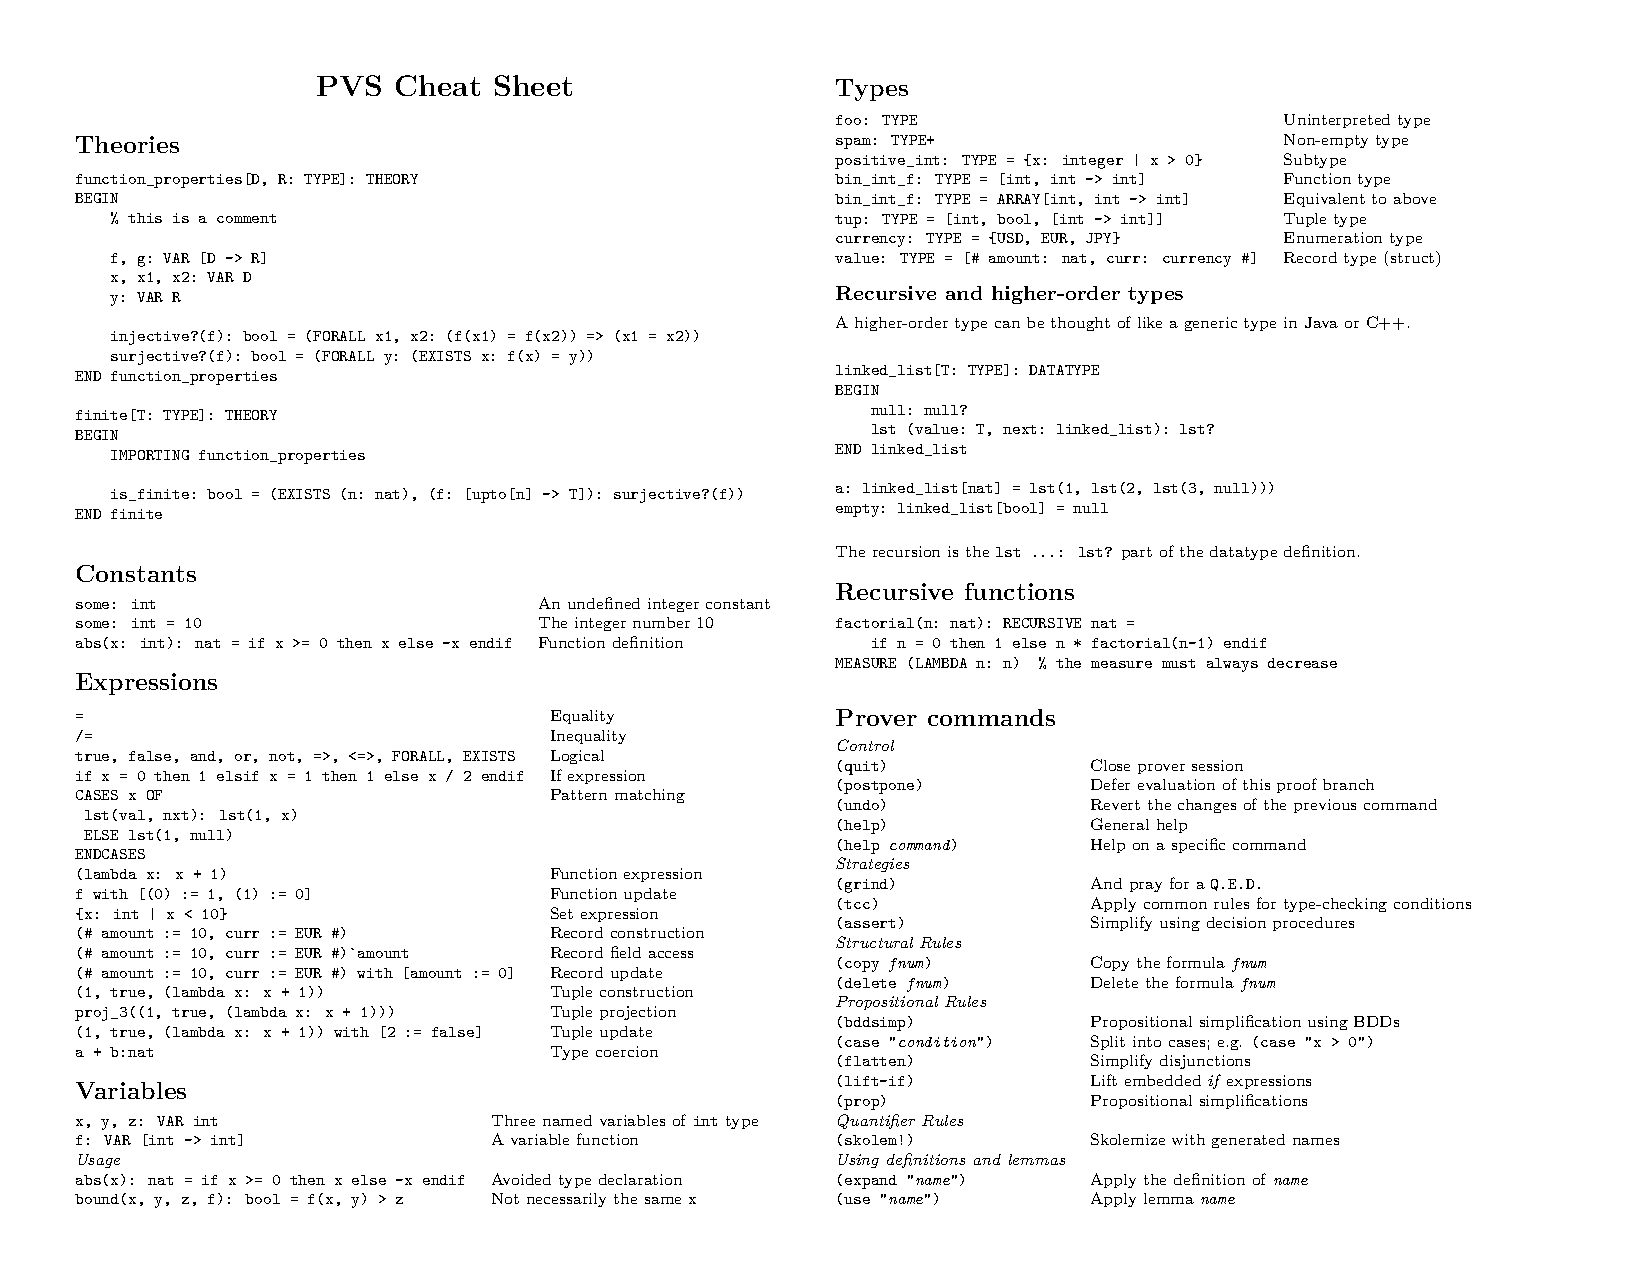
\includepdf[angle=90]{cheatsheet/pvs-cheatsheet.pdf}


\end{document}          
